\documentclass[a4paper,UKenglish]{lipics-v2016}
%This is a template for producing LIPIcs articles. 
%See lipics-manual.pdf for further information.
%for A4 paper format use option "a4paper", for US-letter use option "letterpaper"
%for british hyphenation rules use option "UKenglish", for american hyphenation rules use option "USenglish"
% for section-numbered lemmas etc., use "numberwithinsect"
 
\usepackage{microtype}%if unwanted, comment out or use option "draft"
\usepackage{adjustbox}
\usepackage{color}
\def\fixme#1{\typeout{FIXED in page \thepage : {#1}}
%  \bgroup \color{red}{} \egroup}
\bgroup \color{red}{[FIXME: {#1}]} \egroup}

%\graphicspath{{./graphics/}}%helpful if your graphic files are in another directory

\bibliographystyle{plainurl}% the recommended bibstyle

% Author macros::begin %%%%%%%%%%%%%%%%%%%%%%%%%%%%%%%%%%%%%%%%%%%%%%%%
\title{DeepPicar: A Low-cost Deep Neural Network-based Autonomous Car}
\titlerunning{DeepPicar: A Low-cost Autonomous Car}
%optional, in case that the title is too long; the running title should fit into the top page column

%% Please provide for each author the \author and \affil macro, even when authors have the same affiliation, i.e. for each author there needs to be the  \author and \affil macros
\author[1]{Michael G. Bechtel}
\author[2]{Elise McEllhiney}
\author[3]{Minje Kim}
\author[4]{Heechul Yun}
\affil[1]{University of Kansas, Lawrence, United States\\
  \texttt{mbechtel@ku.edu}}
\affil[2]{University of Kansas, Lawrence, United States\\
  \texttt{e908m429@ku.edu}}
\affil[3]{Indiana University, Bloomington, United States\\
  \texttt{e908m429@ku.edu}}
\affil[4]{University of Kansas, Lawrence, United States\\
  \texttt{heechul.yun@ku.edu}}
\authorrunning{M.\,G. Bechtel, E. McEllhiney, H. Yun} %mandatory. First: Use abbreviated first/middle names. Second (only in severe cases): Use first author plus 'et. al.'

\Copyright{Michael G. Bechtel, Elise McEllhiney, Heechul Yun}%mandatory, please use full first names. LIPIcs license is "CC-BY";  http://creativecommons.org/licenses/by/3.0/

\subjclass{C.4 PERFORMANCE OF SYSTEMS}% mandatory: Please choose ACM 1998 classifications from http://www.acm.org/about/class/ccs98-html . E.g., cite as "F.1.1 Models of Computation". 
\keywords{Real-time, Autonomous car, Convolutional neural network, Case study}% mandatory: Please provide 1-5 keywords
% Author macros::end %%%%%%%%%%%%%%%%%%%%%%%%%%%%%%%%%%%%%%%%%%%%%%%%%

%Editor-only macros:: begin (do not touch as author)%%%%%%%%%%%%%%%%%%%%%%%%%%%%%%%%%%
\EventEditors{Sebastian Altmeyer}
\EventNoEds{1}
\EventLongTitle{30th Euromicro Conference on Real-Time Systems (ECRTS 2018)}
\EventShortTitle{ECRTS 2018}
\EventAcronym{ECRTS}
\EventYear{2018}
\EventDate{July 3--6, 2018}
\EventLocation{Barcelona, Spain}
\EventLogo{}
\SeriesVolume{XX}
\ArticleNo{YY}
% Editor-only macros::end %%%%%%%%%%%%%%%%%%%%%%%%%%%%%%%%%%%%%%%%%%%%%%%
\begin{document}

\maketitle
\thispagestyle{empty}
\begin{abstract}
We present DeepPicar, a low-cost deep neural network (DNN) based
autonomous car platform. DeepPicar is a small scale
replication of a real self-driving car called Dave-2 by NVIDIA, which
drove on public roads using a deep convolutional neural network (CNN), 
that takes images from a front-facing camera as input and produces
car steering angles as output. DeepPicar uses the exact same network
architecture---8 layers, 27 million connections and 250K
parameters---and can be trained to drive itself, in real-time, using a
web camera and a modest Raspberry Pi 3 quad-core platform.
Using DeepPicar, we analyze the Pi 3's computing capabilities to 
support end-to-end deep learning based real-time control of autonomous
vehicles. We also systematically compare other contemporary embedded
computing platforms using the DeepPicar's CNN based real-time control
software as a workload. 
We find all tested platforms, including the Pi 3, are capable of
supporting deep-learning based real-time control, from 20 Hz up to 100
Hz depending on hardware platform. 
However, shared resource contention remains an
important issue that must be considered in applying deep-learning
models on shared memory based embedded computing platforms.
\end{abstract}

%-------------------------------------------------------------------------
\section{Introduction} \label{sec:intro}

% broad context:
% - advance in ai sparked interests in the robotics application, such as
%   self-driving cars.
% - in particular, deep neural network models are increasingly used
%   for perception and control of a vehicle. say. AI workloads.
%
%
Autonomous cars have been a topic of increasing interest in recent
years as many companies are actively developing related hardware
and software technologies toward fully autonomous driving capability with
no human intervention. Deep neural networks (DNNs) have been
successfully applied in various perception and control tasks in
recent years.  They are important workloads for autonomous vehicles
as well. For example, Tesla Model S was known to use a specialized
chip (MobileEye EyeQ), which used a deep neural network for vision-based
real-time obstacle detection and avoidance. More recently, researchers
are investigating DNN based end-to-end control of
cars~\cite{Bojarski2016} and other robots. It is expected that more
DNN based Artificial Intelligence workloads may be used in future
autonomous vehicles.

% big problem
Executing these AI workloads on an embedded computing platform 
poses several additional challenges. First, many AI workloads in vehicles 
are computationally demanding and have strict real-time requirements. 
For example, latency in a vision-based object
detection task may be directly linked to safety of the vehicle. This
requires a high computing capacity as well as the means to guaranteeing
the timings. On the other hand, the computing hardware platform must
also satisfy cost, size, weight, and power constraints, which require a
highly efficient computing platform. These two conflicting
requirements  complicate the platform selection process as observed in
~\cite{Otterness2017}.

%% For example, while today's self-driving car
%% prototype equip more \$100,000
%% of computers and sensors~\cite{juliussen2014emerging}, a study
%% found that aveage consumers are willing to pay much less amount of
%% extra cost for a self-driving capability~\cite{Daziano2017}.
%% https://qz.com/924212/what-it-really-costs-to-turn-a-car-into-a-self-driving-vehicle/

% related work and remaining problems
To understand what kind of computing hardware is needed for AI
workloads, we need a testbed and realistic workloads. While using a real 
car-based testbed would be most ideal, it is not only highly expensive, but also
poses serious safety concerns that hinder development and exploration.
Therefore, there is a strong need for safer and less costly
testbeds. There are already several relatively inexpensive RC-car
based testbeds, such as MIT's 
RaceCar~\cite{shin2017project} and UPenn's F1$/$10 racecar~\cite{upennf1tenth}.
However, these RC-car testbeds still cost more than \$3,000, requiring
considerable investment.

% our goals
Instead, we want to build a low cost testbed that still employs the
state-of-the art AI technologies. Specifically, we focus on a end-to-end
deep learning based real-time control system,
which was developed for a real self-driving car, NVIDIA
DAVE-2~\cite{Bojarski2016}, and use the same methodology on a
smaller and less costly setup. In developing the testbed, our
goals are (1) to analyze real-time issues in DNN based end-to-end
control; and (2) to evaluate real-time performance of contemporary embedded
platforms for such workload.

% DeepPicar introduction
In this paper, we present DeepPicar, a low-cost autonomous car
platform for research. From a hardware perspective,
DeepPicar is comprised of a Raspberry Pi 3 Model B quad-core
computer, a web camera and a RC car, all of which are affordable
components (less than \$100 in total).
The DeepPicar, however, employs state-of-the-art AI
technologies, including a vision-based end-to-end control system that
utilizes a deep convolutional neural network (CNN).
The network receives an image frame from a single forward
looking camera as input and generates a predicted steering angle
value as output at each control period in \emph{real-time}.
The network has 8 layers, about 27 million connections
and 250 thousand parameters (weights).
The network architecture is identical to that of NVIDIA's DAVE-2
self-driving car~\cite{Bojarski2016}, which uses a much more powerful
computer (Drive PX computer~\cite{drivepx}) than a Raspberry Pi~3.
We chose to use a Pi 3 not only because it is affordable, but also because it is representative
of today's mainstream low-end embedded multicore platforms found in
smartphones and other embedded devices.

%% Other than the difference in scale (RC car vs. real car), the only other
%% differences between the two systems---from the computing
%% perspective---are that our system is implemented in
%% TensorFlow~\cite{abadi2016tensorflow} and runs on a Raspberry Pi 3
%% whereas NVIDIA's DAVE-2 systems is implemented in Torch
%% 7~\cite{collobert2011torch7} and runs on a Drive PX computer (NVIDIA's
%% automotive specialized computing system~\cite{drivepx}), which is more
%% powerful but also more expensive.

% how we trained (maybe moved to a later section)
We apply a standard imitation learning methodology to train the car to
follow tracks on the ground. We collect data for
training and validation by manually
controlling the RC car and recording the vision (from the webcam
mounted on the RC-car) and the human control inputs. We then train the
network offline using the collected data on a desktop computer, which
is equipped with a NVIDIA GTX 1060 GPU. Finally, the trained network is copied
back to the Raspberry Pi, which is then used to perform inference
operations---locally on the Pi---in the car's main control loop in
real-time. For real-time control, each inference operation must
be completed within the desired control period (e.g., 33.$\overline{\mbox{33}}$ ms
 period for 30 Hz control frequency).
% how we evaluated (in terms real-time performance)

% what are our findings?
Using the DeepPicar platform, we systematically analyze its real-time
capabilities in the context of deep-learning based real-time
control, especially on real-time deep neural network inferencing.
We also evaluated other, more powerful, embedded computing
platforms to better understand achievable real-time performance of
DeepPicar's deep-learning based control system and the impact of
computing hardware architectures.


We find that the DeepPicar is capable of 
completing control loops in under 33.$\overline{\mbox{33}}$ 
ms, or 30 hz, and can do so 100\% of the time.
Other tested embedded platforms, Intel UP and NVIDIA TX2, offer even
better performance, and are capable of supporting deep-learning based 
real-time control up to 100 Hz control frequency on the TX2 when the GPU 
is used. However, in all platforms, shared resource contention remains 
an important issue as we observe up to 11.6X control loop execution time
increase, mostly due to increase in the neural network inferencing
operation, when memory performance intensive applications are
co-scheduled on idle CPU cores.

% contributions
The {\bf contributions} of this paper are as follows:
\begin{itemize}
  \item We present the design and implementation of a
    low-cost autonomous vehicle testbed, DeepPicar, which utilizes
    state-of-the-art artificial intelligence techniques.
  \item We provide an analysis and case-study of real-time issues in the
    DeepPicar.
  \item We systematically compare real-time computing capabilities of
    multiple embedded computing platforms in the context of
    vision-based autonomous driving.
\end{itemize}

The remaining sections of the paper are as follows: Section II 
provides a background of applications in autonomous driving and related works.
 Section III gives an overview of the DeepPicar platform, including the 
high-level system and the methods used for training and inference. 
Section IV presents our evaluation of the platform and how different 
factors can affect performance. Section V gives a comparison between 
the Raspberry Pi 3 and other embedded computing platforms to 
determine their suitably for autonomous driving research. The paper finishes with 
conclusions in Section VI.

\section{Background} \label{sec:background}

\subsection{Deep End-to-End Control}
End-to-end training of deep neural network models is an active
research area in the fields of AI~\cite{Levine2016}.

\begin{figure}[h]
  \centering
  \includegraphics[width=.5\textwidth]{figs/endtoend}
  \caption{Standard robotics control vs. DNN based end-to-end
    control. \fixme{figure must be redrawn}}
\end{figure}

- explosion of AI
- in particular, application of DNN in perception and control of robotics systems.
- end-to-end control is a promising technique.
  levine's publications?
- examples: nvidia's DAVE-II prototype, forest navigating drone
challenge problem: computing at low cost?

%% UPenn's f1/10 BOM: $3,628.37	
%% http://f1tenth.org/
%% http://selfdrivingcars.mit.edu/
%% http://fast.scripts.mit.edu/racecar/
%% https://github.com/mit-racecar
%% https://mit-racecar.github.io/

\subsection{Embedded Multicore Single-Board-Computers}

- computing has been a obstacle.
- performance, but also constraints size, weight, and power as well as
cost senstive nature of industries including automtive.
- many new embeded computing platforms emerged: affordable and
powerful. raspberry pi, nvidia's embedded platforms tout their
superiority in GPU based acceleration of the AI tasks.

Our primary objective of this study are
- to understand the necessary computing performance for applying AI
technology based robotics systems, and 
- what kind of computing architecture and runtime supports
are most appropriate for such workload.

Toward to achieve the two goals, we implement a low-cost autonomous
car platform as a case study, as we will explain in the following
section. 

\section{DeepPicar Overview}

\begin{figure}[h]
  \centering
  \includegraphics[width=.4\textwidth]{figs/DeepPicar_platform}
  \caption{DeepPicar platform.}
  \label{fig:overview}
\end{figure}

In this section, we provide an overview of our DeepPicar platform. In
developing DeepPicar, one of our primary goals is to replicate the
NVIDIA's DAVE-2 system on a smaller scale with using a low cost
multicore platform, Raspberry Pi 3. Because Pi 3's computing
performance is much lower than that of the DRIVE PX platform, used in
DAVE-2, we are interested in if and how we can process
computationally expensive neural network operations in
real-time. Specifically, inferencing (forward pass processing)
operation must be completed within each control period
duration---e.g., WCET of 50ms for 20Hz control frequency---locally on
the Pi 3 platform, although training of the network (back-propagation
for weight updates) can be done offline and remotely using a desktop
computer.

Figure~\ref{fig:overview} shows the DeepPicar, which is comprised of a
set of inexpensive components: a Raspberry Pi 3 Single Board Computer
(SBC), a Pololu DRV8835 motor driver, a Playstation Eye Webcam, a
battery, and a 1:24 scale RC car. Table~\ref{tbl:carbom} shows
estimated cost of the system.

\begin{table}[h]
  \centering
  \begin{tabular}{|l|l|}
    \hline
    Item                    & cost (\$) \\
    \hline
    Raspberry Pi 3 Model B  & 35 \\
    New Bright 1:24 scale RC car       & 10 \\
    Playstation Eye camera  &  7 \\
    Pololu DRV8835 motor hat&  8 \\
    External battery pack   & 10 \\
    \hline
    Total                   & 70 \\
    \hline
  \end{tabular}
  \caption{DeepPicar's bill of materials (BOM)}
  \label{tbl:carbom}
\end{table}

For the neural network architecture, we adopt a tensorflow version of
NVIDIA's DAVE-2 convolutional neural network (CNN), published by
Fridman at  MIT~\footnote{https://github.com/lexfridman/deeptesla}. As
in NVIDIA's DAVE-2, the CNN takes raw color image (200x66 RGB pixels)
as input and produce a single steering angle value as
output. Figure~\ref{fig:architecture} shows the network architecture, which
is comprised of 9 layers, 250K parameters, and about 27 million
connections.

\begin{figure}[h]
  \centering
  \includegraphics[width=.4\textwidth]{figs/architecture}
  \caption{DeepPicar's neural network architecture: 9 layers (5
    convolutional, 4 fully-connected layers), 250K
    parameters. Adopted from ~\cite{Bojarski2016}.}
  \label{fig:architecture}
\end{figure}

% data collection and training.
To collect the training data, a human pilot manually drives the RC car
on a small track we created (Figure~\ref{fig:track}) to record
timestamped video and contol commands. The stored data is then copied 
to a desktop computer, which equips a NVIDIA GTX 1060 GPU, where we
train the network to accerate training speed. 
For comparison, training the network on the Raspbeery Pi 3 takes
approximately 4 hours, whereas it takes only about 5 minutes on the
desktop computer using the GTX 1060 GPU.

\begin{figure}[h]
  \centering
  \includegraphics[width=.4\textwidth]{figs/track_new2}
  \caption{A track for training/testing.\fixme{replace this}}
  \label{fig:track}
\end{figure}


% inferencing on pi3
Once the network is trained on the desktop computer, the trained model
is copied back to the Raspberry Pi computer. The network is then used
by the car's main controller, which feeds an image frame the web
camera as input to the network. The produced steering angle output is
then converted as the PWM value of the steering motor of the
car. Figure~\ref{fig:controlloop} shows simplified psuedo code of the
controller's main loop.

\begin{figure}[t]
   \lstset{language=python,
           basicstyle=\ttfamily\small,
           keywordstyle=\color{blue}\ttfamily,
           stringstyle=\color{red}\ttfamily,
           commentstyle=\color{green}\ttfamily
          }  
  \lstinputlisting[language=python]{control.py}
  \caption{Control loop}
  \label{fig:controlloop}
\end{figure}

\fixme{Discuss the limitation of the RC car platform: discrete
  control, web camera latency}

%% Although the steering angle output of the network is a continuous
%% real value,

%% We employ a small and relatively inexpensive RC car that is capable of
%% performing basic automotive operations. However, the car we use
%% doesn't replicate the capabilities of other autonomous vehicle
%% platforms, as it is more simplistic in nature. Notably, the RC car we
%% use only has three possible options in terms of turning: center, left,
%% and right. As such, control of the car may be less precise at times,
%% and may negatively affect performance. The car is capable of other
%% operations that aren't used within the scope of this
%% platform. Specifically, the car is able to drive in reverse and the
%% driving speed can be changed. In our experiments, we have the RC car
%% drive forward, and at a constant speed. 

%% Our platform also comes equipped with a camera that is used for both
%% recording training videos and providing input frames to the model
%% whenever the Picar is self-driving. We chose the Playstation Eye
%% Camera due to its ability to reach and maintain higher fps levels
%% while also remaining relatively low-cost. One concern, however, is the
%% affect of camera latency on the self-driving performance of our
%% platform. While humans are able to see environmental changes in
%% real-time, the same can't be said for cameras since there is a delay
%% between when frame capture by the camera, and when it is read by the
%% Raspberry Pi 3. As a result, it is possible for the model to be given
%% an input frame that is different from the real world, thus impacting
%% the performance of the Picar.

%% Compared to other existing autonomous vehicle platforms, such as the
%% F1/10 and NVIDIA DAVE-2, the Picar platform is capable of performing
%% the same operations while using more cost inexpensive components. As
%% shown by Table 1, the components selected for the Picar all cost
%% considerably less than the other  platforms when focusing on the
%% common components (camera, power supply, etc.). Including the other
%% components used in the F1/10 and DAVE-2, such as the additional
%% sensors employed by both, the difference  in cost would be even
%% greater.

%% \subsection{Model Training}
%% In order to operate the Picar as an autonomous vehicle, we utilize the
%% DeepTesla library, which is capable of training a deep neural network
%% (DNN) with end-to-end learning, that could then be used by the  Picar
%% for autonomous driving. Please note that it is more efficient to
%% execute the actual model training  process on a different system with
%% an NVIDIA GPU, rather than on the Raspberry Pi 3 itself. This is
%% because DeepTesla trains the DNN with the Tensorflow library, which
%% greatly benefits from the use of  gpu-enabled operations. For
%% comparison, training a model on the Pi took approximately 6 hours,
%% whereas  the time it took on a computer with a NVIDIA GPU was only
%% around 5 minutes!

%% We train our model on a custom made track/lane composed of black and
%% white duct tape, where the black  tape represents the bounds of the
%% track, and the white tape marks the center of the lane. The model is
%% taught to stay close to the center of the lane for as long as
%% possible, and to turn whenever it  reaches/crosses the outer lane
%% bounds so that it remains on the track. For data, we navigate and
%% record  the car going both ways across the track, and use the
%% collected videos to train the model(s) that will  be used later for
%% angle prediction while the car is self-driving.

%% \begin{table*}[h]
%%   \centering
%%   \begin{tabular} {| l | l | l | l | l |}
%%     \hline
%%     \textbf{Platform} & \textbf{Picar} & \textbf{F1/10} & \textbf{NVIDIA DAVE-2}\\ \hline  
%%     Car & Mini RC Car (\$10) & Traxxas 1/10th car platform (\$299.97) & TBD\\ \hline
%%     Embedded system & Raspberry Pi 3 Model B (\$35.00) & NVIDIA Jetson TK1 (\$192.99) & NVIDIA DRIVE PX \\ \hline
%%     CPU & Cortex A-53 quad core & Cortex A-15 quad core & 8x Cortex A-57 quad core, 8x Cortex A-53 quad core \\ \hline
%%     Camera & Playstation Eye camera (\$6.99) & ZED camera (\$449.00) & 3x cameras\\ \hline
%%     Power Supply & Mobile battery (\$5.99) & Energizer battery pack (\$159.00) & TBD\\
%%     \hline
%%   \end{tabular}
%%   \caption{Comparison of components used in autonomous vehicle platforms.}
%% \end{table*}



\section{Evaluation}\label{sec:evaluation}

In this section, we experimentally analyze various real-time aspects
of the DeepPicar. This includes
(1) measurement based worst-case execution time (WCET) analysis of
deep learning inferencing,
(2) the effect of using multiple cores in accelerating inferencing,
(3) the effect of co-scheduling multiple deep neural network models,
and 
(4) the effect of co-scheduling memory bandwidth intensive co-runners.

\subsection{Setup}

The Raspberry Pi 3 Model B platform used in DeepPicar equip a Boardcom
BCM2837 SoC, which has a quad-core 64bit ARM Cortex-A53 cluster,
running at up to 1.2GHz. The chip also includes Broadcom's Videocore IV
GPU, although we did not use the GPU in our evaluation due to the lack
of sofware support (Tensorflow is not compatible with the GPU).
For software, we use Ubuntu MATE 16.04, Tensorflow 1.1 and python
2.7. We disabled DVFS (dynamic voltage frequency scaling) and
configure the clock speed of each core at the maximum 1.2GHz.

\subsection{Inference Timing for Real-Time Control}

For real-time control of a car (or any robots), the control loop
frequency must be sufficiently high so that the car can quickly
react to the changing environment and its internal states. In general,
control performance improves when the frequency is higher, though
computation time and the type of particular physical system are
factors in determining a proper control loop latency. While a standard
control system may be comprized of multiple control loops with
differning control frequencies---e.g., a inner control loop for lower-level
PD control, a outer loop for motion planning, etc.---DeepPicar's
control loop is a single layer, as shown earlier in
Figure~\ref{fig:controlloop}, as a single deep neural network
replaces the traditional multi-layer control pipline. (Recall
Figure~\ref{fig:end-to-end-control} on the differences between the
standard robotics control vs. end-to-end deep learning approach).
This means that the DNN interference operation must be completed
within the inner-most control loop update frequency. To understand
achievable control-loop update frequencies, we experimentally measured
the execution times of DeepPicar's DNN inference operations.

% 50-200Hz for quadcopters:
% https://robotics.stackexchange.com/questions/231/what-frequency-does-my-quadcopter-output-sense-calculate-output-update-loop-need 
% https://quadmeup.com/pid-looptime-why-it-is-not-only-about-frequency/

\begin{figure}[t]
  \centering
  \includegraphics[width=.45\textwidth]{Total_Processing_Time}
  \caption{DeepPicar's control loop processing times over 1000 input image frames.}
  \label{fig:control-loop-timing}
\end{figure}

\begin{table}[t]
  \centering
  \begin{tabular} {| c | r | r | r | r |}
    \hline
    \textbf{Operation} & \textbf{Mean} & \textbf{Max} &   \textbf{99pct.} & \textbf{Stdev.} \\ \hline
    Image capture        & 2.28  &  4.94 &  4.54  & 0.52 \\ \hline
    Image pre-processing & 3.09  &  4.60 &  3.31  & 0.10 \\ \hline
    DNN inferencing      & 37.30 & 51.03 & 45.48  & 2.75 \\ \hline
    Total Time           & 42.67 & 56.37 & 50.70  & 2.80 \\ \hline
  \end{tabular}
  \caption{Control loop timing breakdown.}
  \label{tbl:control-loop-breakdown}
\end{table}

Figure~\ref{fig:control-loop-timing} shows the measured control loop 
processing times of the DeepPicar over 1000 image frames (one per each
control loop). We omit the first frame processing time for cache
warmup. Table~\ref{tbl:control-loop-breakdown} shows the time
breakdown of each control loop. Note that all four CPU cores of the
Raspberry Pi 3 were used by the Tensorflow library when performing the
DNN inference operations.

First, as expected, we find that the inference operation
dominates the control loop execution time, accounting about 85\% of
the execution time.
Second, more importantly, we also find that the measured average
execution time of a single control loop is 42.67 ms, or 23.4 Hz and
the 99 percentail time is 50.70ms.
This means that the DeepPicar can operates
at about 20 Hz control frequency in real-time using only the on-board
Raspberry Pi 3 computing platform, without needing any remote computing
resources. We consider these results respectable given the complexity
of the deep neural network  and the fact that the inference operation
performed by Tensorflow only utilizes the CPU cores of the
Raspberry Pi 3 (its GPU is not supported by Tensorflow.)

In comparison, NVIDIA's DAVE-2 system, which has the exact same neural
network architecture, is reportedly run at 30 Hz~\cite{Bojarski2016},
just a bit faster than the DeepPicar. Although we believe it was not
limited by their computing platform (we will experimentally compare
performance differences among multiple embedded computing platforms,
including NVIDIA's Jetson TK2, later in
Section~\ref{sec:eval-platforms}), the fact that the low-cost
Raspberry Pi 3 can achieve similar real-time control performance is
surprising.

\subsection{Effect of the Core Count to Inference Timing}

In this experiment, we investigate the scalability of performing
inference operation of DeepPicar's nueral network with respect to the
number of cores. As noted earlier, the Raspberry Pi 3 platform has
four Cortex-A53 cores and the Tensorflow 
provides a programmable mechanism to to adjust how many cores to be
used by the library. Leveraging this feature, we repeat the
same experiment described in the previous subsection with varying
number of CPU cores---from one to four.


\begin{figure}[h]
  \centering
  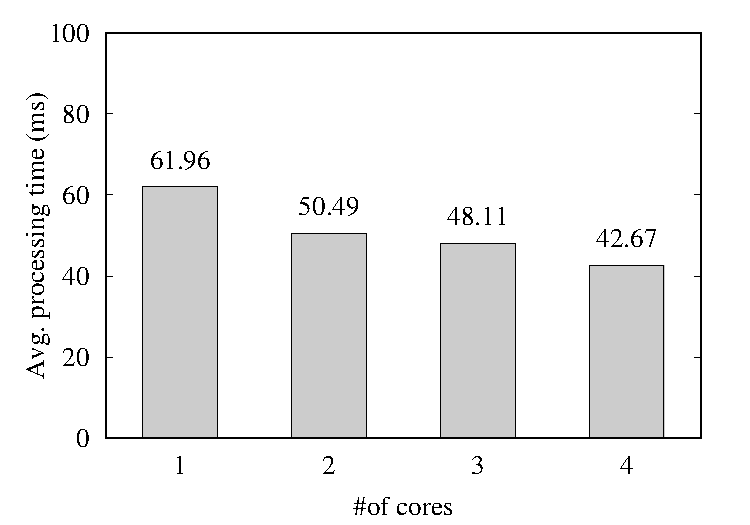
\includegraphics[width=.45\textwidth]{figs/perf_vs_corecnt}
  \caption{Average control loop execution time vs. \#of CPU
    cores. \fixme{instead of the total control loop time, use the
      average of DNN inferencing time.}}
  \label{fig:perf-vs-corecnt}
\end{figure}

%% \begin{table}[h]
%%   \centering
%%   \begin{tabular} {| c | l | l | l | l | l | l | l | l | l |}
%%     \hline
%%     \textbf{\#of cores} & \textbf{Mean} & \textbf{Max} & \textbf{99pct} & \textbf{Stdev} \\ \hline 
%%     1 & 61.96 & 66.00 & 63.31 & 0.51\\ \hline
%%     2 & 50.49 & 71.55 & 70.03 & 3.16 \\ \hline
%%     3 & 48.11 & 72.22 & 58.45 & 4.18 \\ \hline
%%     4 & 42.67 & 56.37 & 50.70 & 2.80 \\
%%     \hline
%%   \end{tabular}
%%   \caption{Execution time statistics vs. \#of CPU cores.}
%% \end{table}

Figure~\ref{fig:perf-vs-corecnt} shows the average execution times of
the control loop as we vary the number of cores used by the
Tensorflow. As expected as we assign more cores, the average execution
time decreases---from 61.96 ms on a single core to 42.67 ms on four
cores. However, the improvement is far from being ideal as we expected
linear scaling. In particular, from 2 cores to 3 cores, the
improvement is mere 2.38ms (or 4\%). In short, we find that the
scalability of DeepPicar's deep neural network is not ideal on the
platform. We do not know whether it is due to the limitations of
Tensorflow's multicore implementation or it's the model's inherent
characteristics. 

The poor scalability opens up the possibility of consolidating
multiple different tasks or different nueral network models rather
than allocating all cores for a single nueral network model. For
example, it is conceivable to use four cameras and four different
neural network models, each of which is trained seperately and
executed on a single dedicated core. Assuming we use the same network
architecture for all models, then one might exepct to achieve up to
15 Hz using one core (given 1 core can deliver 62ms average
execution time). In the next experiment, we investigate the
feasibility of such a scenario.

%% It may not always be the case that all four cores of the Raspberry Pi
%% 3's Cortex A-53 CPU can be used solely for the purpose of operating an
%% autonomous vehicle. Thus, we test how the number of cores utilized for
%% real-time operations affects the DeepPicar's overall ability to
%% function as an autonomous vehicle platform.

%% The performance of the DeepPicar is summarized in Table III. The
%% DeepPicar performed better, on average, when it utilized more
%% cores. With 4 cores, it was able to meet the vast majority of its
%% deadlines, doing so in almost 99\% of the input frames. The platform
%% performed the worst when using only 1 core, as it was unable to meet
%% any of its deadlines.  On average, using 3 cores instead of 2 only had
%% a performance increase of approximately 2 ms, so the addition of one
%% core in that specific case offers  relatively little improvement. One
%% important observation is that the performance was more consistent when
%% only 1 core was used. As a result, the use of multiple cores is very
%% beneficial in terms of reducing the time it takes to complete
%% inference operations, but may result in times that are more volatile.

\subsection{Effect of Co-scheduling Multiple DNN Models}

We also test the capability of the DeepPicar to run multiple models at
the same time, and whether each model can successfully perform within
the given deadline. Specifically, the platform is tested in the cases
of running 2 and 4 models simultaneously. For each case, all models
are allocated an equal number of cores. That is, 2 models are given 2
cores each and 4 models are given 1 core each.

\begin{figure}[h]
  \centering
  \includegraphics[width=.45\textwidth]{figs/perf_vs_modelcnt}
  \caption{Timing impact of co-scheduling multiple DNNs. X-axis shows
    the system configuration: \#of DNN models x \#of CPU cores\/DNN. For
    example, '4x1' means running four DNN models each of which is
    assigned to run on one CPU core, where as '2x2' means running two DNN
    models, each of which is assigned to run on two CPU cores.}
  \label{fig:perf-vs-multimodel}
\end{figure}

%% \begin{figure}[h]
%%   \centering
%%   \includegraphics[width=.5\textwidth]{figs/2ModelChart}
%%   \caption{ Change in inferencing time when 2 models are run concurrently. }
%% \end{figure}

\begin{table}[h]
\centering
  \begin{tabular} {| l | l | l |}
  \hline
  \textbf{num models} & 1 & 2 \\ \hline
  \textbf{L1 refs} &  3.04E+10 &  3.04E+10 \\ \hline
  \textbf{L1 misses} & 4.78E+08 & 4.91E+08 \\ \hline
  \textbf{L1 miss \%} & 1.58 & 1.61 \\ \hline
  \textbf{L2 refs} & 3.31E+09 &  3.91E+09 \\ \hline
  \textbf{L2 misses} & 3.68E+08 & 4.62E+08 \\ \hline
  \textbf{L2 miss \%} & 11.12 & 10.88 \\ \hline
  \end{tabular}
  \caption{ Effect of 2 simulatneous models on cache accesses. }
\end{table}

The results for the 2 model test are outlined in Figure 3 and Table IV, and the 4 model test is summarized in 
Figure 4 Table V. In the the 2 model test, both of the models showed average inference time increases of around 
5-7 ms, $\sim$10\%, when compared to a baseline of 1 model running on two cores. The difference was even 
greater in the 4 model test, as each model displayed an average inference time increase of 
approximately 15 ms, $\sim$30\%, when compared to a single model running on 1 core.

The increase in inference times, however, was not the result of increased cache misses due to 
additional accesses. For all models, the number of L1 misses was always $\sim$1.6\% of all 
references. In the 2 model test, L2 cache misses remained at $\sim$11\% of all references, and each 
model in the 4 model test missed $\sim$13\% of all L2 references.

\begin{figure}[h]
  \centering
  \includegraphics[width=.5\textwidth]{figs/4ModelChart}
  \caption{Change in inferencing time when 4 models are run simultaneously. }
\end{figure}


\begin{table}[h]
\centering
  \begin{tabular} {| l | l | l |}
  \hline
  \textbf{num models} & 1 & 4 \\  \hline
  \textbf{L1 refs} & 2.78E+10 & 2.79E+10 \\ \hline
  \textbf{L1 misses} & 4.36E+08 & 4.53E+08 \\ \hline
  \textbf{L1 miss \%} & 1.57 & 1.63 \\ \hline
  \textbf{L2 refs} & 2.83E+09 & 3.36E+09 \\ \hline 
  \textbf{L2 misses} & 3.59E+08 & 4.43E+08 \\ \hline
  \textbf{L2 miss \%} & 12.68 & 13.19 \\ 
\hline
  \end{tabular}
  \caption{ Effect of 4 concurrent models on cache accesses. }
\end{table}

In all multimodel tests, it was found that a greater number of models run simultaneously resulted in 
interference that led to a noticable increase in the average inferencing time that wasn't 
attributable to a change in cache misses. Instead, the overall time increases can most likely be 
traced to an increase in cache latency. Even if the models had a consistent number of cache hits, it 
is highly probable that the contention for the cache increased the access time for each model, 
consequently increasing the time it took for the models to execute their operations.

In terms of real-time performance under a WCET of 50 ms, the DeepPicar was unsatisfactory in all 
multimodel tests. On average, the 2 model test saw models miss their deadline by 6-8 ms, and the 4 
model test was worse as each model went over their deadlines by 27-29 ms. As a result, it can be 
ascertained that, if a WCET of 50 ms is required, DeepPicar would not be able to perform as necessary.

\subsection{Benchmark Performance}
In order to determine how cache misses affects the performance of the DeepPicar, we test its ability by 
running synthetic benchmarks concurrently with the model. In each experiment, we run a single model on a 
number of cores, and a synthetic benchmark on the remaining idle cores. The effects of the benchmarks can
seen in Figure 9 and Table VI.

\begin{figure}[h]
  \centering
  \includegraphics[width=.5\textwidth]{figs/BenchmarkChart}
  \caption{ Effect of benchmarks on inferencing time. }
\end{figure}

\begin{table}[h]
\centering
  \begin{tabular} {| l | l | l | l | l | l |}
  \hline
  \textbf{num cores} & 1 & 2 & 3 \\ \hline
  \textbf{L1 refs} & 3.16E+10 & 3.17E+10 & 3.06E+10 \\ \hline
  \textbf{L1 misses} & 5.41E+08 & 5.35E+08 & 4.98E+08 \\ \hline
  \textbf{L1 miss \%} & 1.71 & 1.69 & 1.62 \\ \hline
  \textbf{L2 refs} & 3.49E+09 & 3.23E+09 & 3.21E+09 \\ \hline
  \textbf{L2 misses} & 8.05E+08 & 7.54E+08 & 4.98E+08 \\ \hline
  \textbf{L2 miss \%} & 23.05 & 23.37 & 15.51 \\ 
  \hline
  \end{tabular}
  \caption{ Effect of benchmarks on cache accesses. }
\end{table}

The presence of the benchmark(s) had a noticable effect on the DeepPicar, with all tests showing 
increases in inferencing operations. The least change happened when the model was run on 3 cores, and a 
single benchmark was run on the final core. Even with a slight increase in the number of L2 cache 
misses, inferencing was able to be completed in under 100 ms. The other tests, however, showed dramatic 
changes when the model was run on 1 and 2 cores. In both instances, L2 misses rose to $\sim$23\% of all 
references. The additional benchmark in the 1 core test was even more detrimental as the average 
inferencing time was at least 150 ms longer than when the model used 2 cores. 

With the introduction of synthetic benchmarks, the DeepPicar failed to comply with the 50 ms WCET across 
all tests run. Even in the best case, inferencing operations take twice as long as the deadline to 
complete. As a result, if benchmarks were required to run during autonomous operation, the DeepPicar 
wouldn't be capable of meeting its deadlines.

\subsection{Summary}
We found that the DeepPicar is capable of successfully completing all necessary inferencing 
operations within a given deadline of 50 ms. Between these operations, it was discovered that the 
angle prediction time of the model was the dominating step in the processing time of a single frame. 
The other operations were found to execute in very little time, with either one taking 5 ms at most.

When running a single model, DeepPicar performed the best when it used all 4 cpu cores, as it was 
able to process a frame in 43 ms on average. This feat can still be accomplished when running a 
single model on 3 cpu cores, and is also possible when using 2 cores. The only time in which the Pi 
can't run a single model under 50 ms is when only 1 core is used. This was also the case when 
multiple models were run concurrently as no models were able to consistently complete inference 
operations in under 50 ms.

However, the DeepPicar was shown to be capable of handling other potential WCETs. If given a larger 
deadline, the capabilities of DeepPicar as an autonomous vehicle platform would be greatly increased. 
For example, if tested with a deadline of 66.67 ms, or 15 fps, the platform would have passed several 
of the experiments performed. In actuality, the DeepPicar would have only been unsatisfactory in the 
4 model test where it would have missed the deadlines by $\sim$10 ms, and the benchmark tests, where 
it would still miss by $\sim$33 ms at best.

\subsection{Performance Requirements}
In the utilization of the Raspberry Pi 3 in our platform, there are a few factors that need to be 
considered and/or enforced in order to guarantee that the Pi is able to consistently perform at a 
desired level. Specifically, these issues all have the potential to negatively affect the cpu clock 
speed/frequency, which would result in decreased performance. While, in the above experiments, the cpu 
operated at a preferred clock speed of 1.2 GHz, it is entirely possible for the cpu to operate at a 
lower frequency if the following problems are not taken into account.

The most notable issue that can affect the cpu clock speed is that of the power supplied to the 
Raspberry Pi. In essence, it is necessary that the Pi be supplied with 2 Amps, as any less could 
hinder the Pi's ability to maintain a 1.2 GHz frequency. In experiments conducted with a power supply that 
only provided 1 Amp, the Pi was unable to sustain a 1.2 GHz clock speed and, instead, fluctuated 
between operating at 600 MHz and 1.2 GHz. As a result, it is necessary, or at least highly 
recommended, that the power supply used for the Raspberry Pi 3 be capable of outputting 2 Amps, 
otherwise optimal performance isn't guaranteed.

Another factor that can affect clock speed is that of the cpu's temperature. Some model operations can 
be computationally intensive, thus it is possible for the temperature of the cpu to become relatively 
high. This can be especially problematic in situations where multiple models are running 
simultaneously on the Pi. Consequently, thermal throttling may be used to decrease the clock 
speed so that the cpu temperature stays at a safe level. Thus the Raspberry Pi may not be suited 
for prolonged use, especially in cases where the workload is relatively larger, such as running multiple 
models. Rather, the Pi seems to be better suited for running in set periods, after which it is turned 
off or made idle so that the cpu is allowed time to cool down.

\subsection{System Comparisons}
We compare the real time performance of the Raspberry Pi 3 to two other embedded computing platforms, 
the Intel UP Board the NVIDIA Tegra TX2, to evaluate their efficacy in vision-based autonomous 
vehicles. We conduct the same experiments done on the DeepPicar with each platform, and analyze the 
results.

\begin{figure}[h]
  \centering
  \includegraphics[width=.5\textwidth]{figs/system_multicore}
  \caption{Inferencing time across platforms based on number of cores used.}
  \label{fig:sys_core}
\end{figure}

The results of the multicore tests can be seen in Figure~\ref{fig:sys_core}. It was found that the 
Intel UP Board performed better in all experiments. On average, it was able to perform inferencing 
operations, at least, twice as fast as the Raspberry Pi 3. As a result, the UP Board was able to 
satisfy the 50 ms WCET by a very clear margin (in the worst case, it would still meet it by $\sim$20 
ms), and, thus, demonstrates that it is more capable of autonomous driving than the Raspberry Pi 3.

The Intel UP Board also performed better in the multimodel tests, as is shown in 
Figure~\ref{fig:sys_model}. Once again, the UP was able to complete inferecing operations in half the 
time when compared to the Pi. Furthermore, the Intel UP Board was capable of satisfying the 50 ms 
WCET, while the Raspberry Pi 3 was unable to do so. As such, the Intel UP Board displays greater 
potential for the simultaneous execution of multiple models during self-driving operation, while the 
Raspberry Pi 3 would struggle to do so.

\begin{figure}[h]
  \centering
  \includegraphics[width=.5\textwidth]{figs/system_multimodel}
  \caption{Inferencing time across platforms based on number of models run concurrently.}
  \label{fig:sys_model}
\end{figure}

Finally, we examined if the performance of the Intel UP Board and Tegra TX2 would be affected by the 
addition of the synthetic benchmarks. As summarized in Figure~\ref{fig;sys_bench}, the Intel UP Board 
did experience a change in its inferencing times, but the increase was not as drastic as is seen by 
the Raspberry Pi 3. in the worst case, the Intel UP Board produced times that were over two times as 
large, whereas the Raspberry Pi 3 output times that were around 10 times greater. The Intel UP Board 
was successful in completing inferencing operations in under 50 ms when benchmarks were run on a 
maximum of 2 cores, while the Raspberry Pi 3 failed to do so when any benchmark was introduced. As 
such, it can be concluded that the Intel UP Board would be more capable of running computationally 
heavy processes during autonomous driving, and that the Pi wouldn't be able to do the same.

\begin{figure}[h]
  \centering
  \includegraphics[width=.5\textwidth]{figs/system_benchmark}
  \caption{Inferencing time across platforms based on number of cores used.}
  \label{fig:sys_bench}
\end{figure} 

In the comparison of the real-time capabilities of three embedded computing platforms, we found that 
the Raspberry Pi 3 performed the worst. When compared to the Intel UP Board, inferencing on the Pi 
took twice as long across all multicore and multimodel experiments. The difference was even more 
noticeable in the the addition of computationally heavy synthetic benchmarks that had a much more 
dire effect on the Pi.




%% In our platform, three main real-time tasks are performed during autonomous operation. In order, these 
%% operations are: (1) capturing and reading the input frame from the designated camera or video stream, 
%% (2) preprocessing the acquired frame so that it is compatible with the DNN, and (3) feeding the frame 
%% to, and getting the angle prediction from, the model. We aim to determine which operation(s), if any, 
%% require the most time to be performed.

%% In order to determine which operation(s) take the longest to execute, we measured the time it 
%% took for each step to be completed. For this experiment, all four of the Pi's cpu cores were utilized, 
%% and only one model was run. As is shown in Table II, the angle prediction operation consumes the 
%% majority of the processing for each frame. Furthermore, the time it takes for the operation to 
%% complete is volatile, and can range anywhere between 30 ms and 50 ms for any particular frame. On the 
%% other hand, both the frame capture and preprocessing operations take substantially less time 
%% and are relatively more consistent in their times, at 2 ms and 3 ms, respectively. 


%% In evaluating the real-time efficacy of the DeepPicar, the methodology is consistent across all 
%% experiments. The performance of the platform is measured over a set of 1001 video frames that are 
%% each individually fed to the model. The processing time for the first frame is omitted as, due to 
%% cache warmup, it is uncharacteristically high and doesn't
%% accurately represent the Picar's capabilities.  
%% A WCET of 50 ms, or 20 Hz, is used as a baseline to assess the platform's ability to complete all 
%% necessary real-time operations in a timely manner.

%% We seek to determine if the DeepPicar is capable of consistently executing all necessary functions 
%% before their given deadlines. In the case of our platform, it has to process every given frame and get 
%% the predicted angles from the model within a WCET of 50 ms. In order to determine if this was achievable, 
%% we tested the platform by running a single model that utilized all 4 cpu cores and measured the time it 
%% took for each frame to be processed. The performance of the DeepPicar can be seen in Figure 6. We found 
%% that DeepPicar was able to completely process the vast majority of the provided frames within 50 ms, and 
%% was unable to do so for very few frames.

%% In our platform, three main real-time tasks are performed during autonomous operation. In order, these 
%% operations are: (1) capturing and reading the input frame from the designated camera or video stream, 
%% (2) preprocessing the acquired frame so that it is compatible with the DNN, and (3) feeding the frame 
%% to, and getting the angle prediction from, the model. We aim to determine which operation(s), if any, 
%% require the most time to be performed.

%% In order to determine which operation(s) take the longest to execute, we measured the time it 
%% took for each step to be completed. For this experiment, all four of the Pi's cpu cores were utilized, 
%% and only one model was run. As is shown in Table II, the angle prediction operation consumes the 
%% majority of the processing for each frame. Furthermore, the time it takes for the operation to 
%% complete is volatile, and can range anywhere between 30 ms and 50 ms for any particular frame. On the 
%% other hand, both the frame capture and preprocessing operations take substantially less time 
%% and are relatively more consistent in their times, at 2 ms and 3 ms, respectively. 


%
% raspberry p3 spec: https://www.raspberrypi.org/magpi/raspberry-pi-3-specs-benchmarks/

\section{Embedded Computing Platform Comparison}\label{sec:comparison}


\begin{table*}[h]
  \centering
  \begin{adjustbox}{width=1\textwidth}
  \begin{tabular}{|c|c|c|c|}
    \hline
    Item    & Raspberry Pi 3 (B)   & Intel UP                  & NVIDIA Jetson TX2\\
    \hline
            & BCM2837              & X5-Z8350 (Cherry Trail)   & Tegra X2 \\
    CPU     & 4x Cortex-A53@1.2GHz/512KB L2  &
              4x Atom@1.92GHz/2MB L2 &
              4x Cortex-A57@2GHz/2MB L2 \\
            &              &              & 2x Denver@2.0GHz/2MB L2 (not used)  \\
    \hline
    GPU     &  VideoCore IV (not used)    &
               Intel HD 400 Graphics (not used) &
               Pascal 256 CUDA cores   \\
    \hline
    Memory  & 1GB LPDDR2   &  2GB DDR3L     & 8GB LPDDR4              \\
    \hline
	Peak Memory Bandwidth & 8.5 GB/s & 12.8 GB/s & 59.7 GB/s \\
	\hline
	Measured Bandwidth & 2127.94 MB/s & 3951.94 MB/s & 4447.90 MB/s \\
	\hline
	Cost (\$) & 35 & 100 & 600 \\
	\hline
  \end{tabular}
  \end{adjustbox}
  \caption{Compared embedded computing platforms}
  \label{tbl:platforms}
\end{table*}

In this section, we compare three computing platforms---the Raspberry
Pi 3, the Intel UP~\footnote{http://www.up-board.org/up/} and the NVIDIA
Jetson
TX2~\footnote{http://www.nvidia.com/object/embedded-systems-dev-kits-modules.html}---from
the point of view of supporting end-to-end deep learning
based autonomous vehicles. 
Table~\ref{tbl:platforms} shows architectural features of the three
platforms~\footnote{The GPU of Intel UP and the two Denver cores in the
  Tegra TX2 are not used in evaluation due to TensorFlow issues.}.
  
Our basic approach is to use the same DeepPicar software, and repeat
the experiments in Section~\ref{sec:evaluation} on each hardware
platform and compare the results. 
%We do not, however, repeat the cache
%partitioned experiments done on the Pi 3, as we did not believe our 
%findings warranted further experimentation on additional platforms. 
For the Jetson TX2, we have two different system configurations,
which differ in whether TensorFlow is configured to use its GPU or
only the CPU cores. Thus, a total of four system configurations are
compared.

\begin{figure}[h]
  \centering
  \includegraphics[width=.7\textwidth]{figs/compare_core}
  \caption{Average control loop execution time.} 
  \label{fig:sys_core}
\end{figure}

Figure~\ref{fig:sys_core} shows the average control loop completion
timing of the four system configurations we tested as a function of
the number of CPU cores used.
First, both the Intel UP and Jetson TX2 exhibit superior performance when
compared with the Raspberry Pi 3. 
When all four CPU cores are used, the Intel UP is 1.33X faster than
the Pi 3, while the TX2 (CPU) and TX2 (GPU) are 2.79X and 4.16X times faster,
respectively, than the Pi 3. 
As a result, they are all able to satisfy the 33.$\overline{\mbox{33}}$ ms 
WCET by a clear margin,
%%  (in the worst case, the UP Board would 
%% still meet it by $\sim$20 ms) --> where's the data showing this?
and, in the case of the TX2, 50 Hz or even 100 Hz real-time control is
feasible with the help of its GPU. Another observation is that the TX2
(GPU) performance does not change much, as most of the neural network 
computation is done at the GPU.

\begin{figure}[h]
  \centering
  \includegraphics[width=.7\textwidth]{figs/compare_model}
  \caption{Average control loop execution time when multiple DNN
    models are co-scheduled. }
  \label{fig:sys_model}
\end{figure}

The Intel UP board and Jetson TX2 also perform much better when multiple DNN models
are co-scheduled. Figure~\ref{fig:sys_model} shows the results of the
multi-model co-scheduling experiment. Once again, they can comfortably
satisfy 30 Hz real-time performance for all of the co-scheduled DNN control
loops, and in the case of the TX2 (GPU), 100 Hz real-time control is still
feasible. Given that the GPU must be shared among the co-scheduled DNN
models, the results suggest that the TX2's GPU has sufficient capacity to
accomodate multiple instances of the DNN models we tested.

\begin{figure}[h]
  \centering
  \includegraphics[width=.7\textwidth]{figs/compare_benchmark}
  \caption{Average control loop execution time in the presence of an
    increasing number of memory intensive applications on idle CPU cores.}
  \label{fig:sys_bench}
\end{figure} 

\begin{figure}[h]
  \centering
  \includegraphics[width=.7\textwidth]{figs/compare_l2missrate}
  \caption{L2 miss rates in the presence of an increasing number of 
			memory intensive applications on idle CPU cores.}
  \label{fig:sys_l2miss}
\end{figure}

Finally, we compare the effect of co-scheduling memory bandwidth
intensive synthetic benchmarks on the DNN control loop timing. 
Figure~\ref{fig:sys_bench} shows the results.
As discussed in 
Section~\ref{sec:eval-memhog}, we observed dramatic execution time
increases, up to 11.5X, in Raspberry Pi 3 as we increased the number of
co-scheduled tasks. We also observe increased control loop execution
timing in the Intel Up and Jetson TX2, but the degree of the increase is 
not as dramatic as the Pi 3. Compared to their respective solo timings 
(i.e., the model runs on a single core in isolation), Intel UP suffers up to
2.3X execution time increase; TX2 (CPU) and TX2 (GPU) suffer up to
2.2X and 2.1X increases, respectively. This is somewhat suprising
because the Raspberry Pi 3's cores are in-order architecture based while
the cores in the Intel Up and NVIDIA TX2 are out-of-order architecture
based, and that the memory intensive tasks on out-of-order cores can
generate more memory traffic. We suspect that this is because the
memory subsystems in the Intel UP and TX2 platforms provide higher
bandwidth and fairness than the memory subsystem of the Pi 3. However, 
the L2 miss rates of the Pi 3 and TX2 platforms follow the same expected 
pattern, as can be seen in Figure~\ref{fig:sys_l2miss}. Namely, the 
percentage of L2 miss rates increases are more 
memory intensive co-runners are introduced. This was not the case for 
the UP board, where the model running on two cores generated the highest
percentage of L2 cache misses. This is most likely due to the CPU 
architecture of the UP's CPU which is Intel based, whereas both the Pi 3
and TX2 have ARM based CPUs.

Another interesting observation is that the TX2 (GPU) also suffers
considerable execution time increase (2.1X) despite the fact that the
co-scheduled synthetic tasks do not utilize the GPU. In other words,
the DNN model has dedicated access to the GPU. This is, however, a
known characteristic of integrated CPU-GPU architectue based
platforms where both CPU and GPU share the same memory
subsystem~\cite{Ali2017}. As a result, the TX2 (GPU) fails to meet the
10ms deadline for 100 Hz control that would have been feasible if
there was no contention between the CPU cores and the GPU.

In summary, we find that today's embedded computing platforms, even as
inexpensive as a Raspberry Pi 3, are powerful enough to support
vision and end-to-end deep learning based real-time control
applications. Furthermore, availability of CPU cores and GPU on these
platforms allow consolidating mutiple deep neural network based AI
workloads. However, shared resource contention among these diverse
computing resources remains an important issue that must be understood
and controlled, especially for safety-critical applications.

\section{Related Work}\label{sec:related}
% discusstion
% - model is still quite small. cam we use bigger CNNs?
%% \fixme{What we want to say:
%%   1) We showed DNN is feasible on today's embedded computing
%%   platforms.
%%   2) But, the CNN model is rather smaller-kind with respect to today's
%%   state-of-the-art CNNs, which are much bigger.
%%   3) disscuss google's object detection api
%%   paper~\cite{huang2017speed}. 
%%   4) Applying these much more complex DNNs (such as google's detection
%%   models) may be challenging for embedded computing
%%   platforms.
%%   5) Two general approaches: (1) make it faster (computing workload
%%   remains the same) (2) reduce the workload itself (model compression
%%   or reduced precision etc.)}

%% {\bf DNN optimization for embedded systems.}

There are several relatively inexpensive RC-car based autonomous car
testbeds. MIT's RaceCar~\cite{shin2017project} and UPenn's
F1$/$10~\cite{upennf1tenth} are both based on a Traxxas 1/10 scale RC
car and a NVIDIA Jetson multicore computing platform, which
is equipped with many sophisticated sensor packages, such as a lidar.
However, they both cost more than \$3,000, requiring a considerable
investment. DonkeyCar~\cite{donkeycar} is similar to our DeepPicar as
it also uses a Raspberry Pi 3 and a similar CNN for end-to-end
control, although it costs more (about \$200).
%% because it uses a more
%% expensive 1/16 scale RC car than our 1/24 scale one.
The main contribution of our paper is in the detailed analysis of
computational aspects of executing a CNN-based real-time control
workload on diverse embedded computing platforms.

In this paper, we have analyzed real-time performance of a real-world
CNN, which was used in NVIDIA's DAVE-2 self-driving
car~\cite{Bojarski2016}, on a low-cost raspberry pi 3 quad-core 
platform and other embedded multicore platforms. It should be noted, 
however, that DAVE-2's CNN is relatively small compared
to recent state-of-the-art CNNs, which are increasingly larger and
deeper. For example, the CNN based object detector models evaluated in
Google's recent study~\cite{huang2017speed} have between 3M to 54M
parameters, and are much larger than DAVE-2's CNN.
Using such large CNN models will be challenging on
resource constrainted embedded computing platforms, especially for
real-time applications such as self-driving cars.

%% available DNN's can be much larger compared to the architecture of the
%% DAVE-2. Such DNN's can be seen in Google's Object Detection API
%% The smallest model available in the API is the MobileNet model, which
%% has 3,191,072 parameters and is approximately 12.7 larger than the
%% model used by the DeepPicar. The other models all have parameter sizes 
%% of at least 10 million. Due to the considerable differences in the 
%% model sizes, it is likely that running them on platforms like the Pi 3,
%% and still get acceptable real-time performance would be difficult, 
%% if not infeasible. 

%% % related work on efficient DNN representation and processing.
%% While repeated feedforward and backpropagation operations during
%% the training time account for most of the computational cost in
%% deep learning, there is a growing need for an improved efficiency
%% during the inferencing time as well, especially because of the
%% potential of utilizing Deep Neural Networks (DNN) for the real-time
%% pattern recognition tasks in embedded systems, as our paper
%% exemplifies.

While continuing performance improvements in embedded computing
platforms will certainly make processing these complex CNNs faster,
another actively investigated approach is to reduce the required
computational complexity itself.
%% When a DNN is deployed in those implementations with limited
%% resources, such as memory and power, the floating-point operations
%% involved in the large matrix multiplications are a burdensome task.
Many recent advances in network compression have shown promising results
in reducing such computational costs during the feedforward
process. The fundamental assumption in those techniques is that the
CNNs are redundant in their structure and representation. For example,
network pruning can thin out the network and provides a more condensed
topology~\cite{han2015deep}.

Another common compression method is to reduce the
quantization level of the network parameters, so that arithmetic
defined with floating-point operations are replaced with low-bit
fixed-point counterparts. To this end, single bit quantization of the
network parameters or ternary quantization have been recently proposed
~\cite{hwang2014fixed,soudry2014expectation,kim2016bitwise,rastegari2016xnor,hubara2016binarized,beauchamp2006embedded,govindu2004analysis}.
In those networks, the inner product between the
originally real-valued parameter vectors is defined with XNOR followed
by bit counting, so that the network can greatly minimize the
computational cost in the hardware implementations. This drastic
quantization can produce some additional performance loss, but those
new binarized or ternarized systems provide a simple quantization
noise injection mechanism during training so that the additional error
is minimized to an acceptable level.

The XNOR operation and bit counting have been known to be efficient in
hardware implementations. In~\cite{rastegari2016xnor}, it was shown
that the binarized convolution could substitute the expensive
convolutional feedforward operations in a regular Convolutional Neural
Network (CNN), %% by using only about 1.5\% of the memory space, while
providing 20 to 60 times faster feedforward. Binary weights were also
able to provide 7 times faster feedforward than a floating-point
network for the hand written digit recognition task as well as 23
times faster matrix multiplication tasks on a
GPU~\cite{hubara2016binarized}.
Moreover, FPGA implementations showed that the XNOR operation is 200
times cheaper than floating-point multiplications with 
single precision~\cite{beauchamp2006embedded,govindu2004analysis}.
XNOR-POP is another hardware implementation that reduced
the energy consumption of a CNN by 98.7\%~\cite{jiang2017xnor}.

These research efforts are expected to make complex CNNs more
accessible for a wider range of real-time embedded systems. We plan to
investigate the feasibility of these approaches in the context of
DeepPicar so that we can use even more resource constrained
micro-controller class computing platforms.

%% % related work on testbeds
%% \fixme{maybe we can also discuss MIT racecar, UPENN car, donkey car and other testbeds?
%%   The points of discussion may include: 1) they are expensive. 2)
%%   donkey car is similar to us, but still a bit more expnsive, and more
%%   importantly there is no existing studies which systematically evaluate
%%   real-time performance of using DNN on embedded computing
%%   platforms. Our work provides quantitive real-time performance
%%   evaluation results, using a known DNN used in a real self-driving
%%   car. Our work is fully reproducible at a very low cost, lowring the
%%   barrier to entry in researching self-driving cars, helping the
%%   community blah blah blah.}
  

%% and the ability of the car to navigate the desired environment. We are 
%% more focused on the real-time performance of the DeepPicar, and whether
%% the Raspberry Pi 3 embedded computing platform can properly support autonomous 
%% vehicle operations. To the best of our knowledge, no other studies have
%% been done to evaluate the capabilities of the Pi 3 for running DNNs and
%% performing autonomous vehicle operations.

\section{Conclusion}\label{sec:conclusion}
We presented DeepPicar, a low cost autonomous car platform that is
inexpensive to build, but is based on state-of-the-art AI technology:
End-to-end deep learning based real-time control.
Specifically, DeepPicar uses a deep convolutional neural network to
predict steering angles of the car directly from camera input data
in real-time. Importantly, DeepPicar's neural network architecture is
identical to that of NVIDIA's real self-driving car. 

Despite the complexity of the neural network, DeepPicar uses a
low-cost Raspberry Pi 3 quad-core computer as a sole computing
resource. We systematically analyzed the real-time characteristics of
the Pi 3 platform in the context of deep-learning based real-time
control appilcations, with a special emphasis on real-time deep neural
network inferencing.
We also evaluated other, more powerful, embedded computing
platforms to better understand achievable real-time performance of
DeepPicar's deep-learning based control system and the impact of
computing hardware architectures.
We find all tested embedded platforms, including the Pi3, are capable
of supporting deep-learning based real-time control, from 20 Hz up to
100 Hz, depending on the platform and its system
configuration. However, shared resource contention remains an
important issue that must be considered in applying deep-learning
models on shared memory based embedded computing platforms.

%% We evaluated the real time efficacy of our platform and found
%% that it is capable of performing inferencing operations within a WCET
%% of 50 ms, or 20 fps, when a single model is run on more than one
%% core.

As future work, we plan to apply shared resource management
techniques~\cite{Yun2013,yun2014rtas} on the DeepPicar platform and
evaluate their impact on the real-time performance of the system. We
also plan to improve the prediction accuracy by feeding more data and
upgrading the RC car hardware platform to enable more precise steering
angle control.

%% Further studies should be conducted on the interference that
%% occurs between cores to allow for improved performance in utilizing
%% multiple models for autonomous vehicles. With minimal further
%% research, the DeepPicar can become a valudable, reliable and
%% inexpensive tool in the continued research of autonomous vehicles.

%-------------------------------------------------------------------------
%\bibliographystyle{abbrv}
\bibliography{reference}

\appendix

\subsection{System-level Factors Affecting Real-Time Performance}
In the utilization of the Raspberry Pi 3 in our platform, there are a
few factors that need to be considered and/or enforced in order to
guarantee that the Pi is able to consistently perform at a desired
level. Specifically, these issues all have the potential to negatively
affect the cpu clock speed/frequency, which would result in decreased
performance. While, in the above experiments, the cpu operated at a
preferred clock speed of 1.2 GHz, it is entirely possible for the cpu
to operate at a lower frequency if the following problems are not
taken into account. 

The most notable issue that can affect the cpu clock speed is that of
the power supplied to the Raspberry Pi. In essence, it is necessary
that the Pi be supplied with 2 Amps, as any less could hinder the Pi's
ability to maintain a 1.2 GHz frequency. In experiments conducted with
a power supply that only provided 1 Amp, the Pi was unable to sustain
a 1.2 GHz clock speed and, instead, fluctuated between operating at
600 MHz and 1.2 GHz. As a result, it is necessary, or at least highly
recommended, that the power supply used for the Raspberry Pi 3 be
capable of outputting 2 Amps, otherwise optimal performance isn't
guaranteed.

Another factor that can affect clock speed is that of the
cpu's temperature. Some model operations can be computationally
intensive, thus it is possible for the temperature of the cpu to
become relatively high. This can be especially problematic in
situations where multiple models are running  simultaneously on the
Pi. Consequently, thermal throttling may be used to decrease the clock
speed so that the cpu temperature stays at a safe level. Thus the
Raspberry Pi may not be suited for prolonged use, especially in cases
where the workload is relatively larger, such as running multiple
models. Rather, the Pi seems to be better suited for running in set
periods, after which it is turned  off or made idle so that the cpu is
allowed time to cool down. 


\end{document}
